% Options for packages loaded elsewhere
\PassOptionsToPackage{unicode}{hyperref}
\PassOptionsToPackage{hyphens}{url}
%
\documentclass[
]{article}
\usepackage{lmodern}
\usepackage{amsmath}
\usepackage{ifxetex,ifluatex}
\ifnum 0\ifxetex 1\fi\ifluatex 1\fi=0 % if pdftex
  \usepackage[T1]{fontenc}
  \usepackage[utf8]{inputenc}
  \usepackage{textcomp} % provide euro and other symbols
  \usepackage{amssymb}
\else % if luatex or xetex
  \usepackage{unicode-math}
  \defaultfontfeatures{Scale=MatchLowercase}
  \defaultfontfeatures[\rmfamily]{Ligatures=TeX,Scale=1}
\fi
% Use upquote if available, for straight quotes in verbatim environments
\IfFileExists{upquote.sty}{\usepackage{upquote}}{}
\IfFileExists{microtype.sty}{% use microtype if available
  \usepackage[]{microtype}
  \UseMicrotypeSet[protrusion]{basicmath} % disable protrusion for tt fonts
}{}
\makeatletter
\@ifundefined{KOMAClassName}{% if non-KOMA class
  \IfFileExists{parskip.sty}{%
    \usepackage{parskip}
  }{% else
    \setlength{\parindent}{0pt}
    \setlength{\parskip}{6pt plus 2pt minus 1pt}}
}{% if KOMA class
  \KOMAoptions{parskip=half}}
\makeatother
\usepackage{xcolor}
\IfFileExists{xurl.sty}{\usepackage{xurl}}{} % add URL line breaks if available
\IfFileExists{bookmark.sty}{\usepackage{bookmark}}{\usepackage{hyperref}}
\hypersetup{
  pdftitle={Gestion de Portefeuille},
  pdfauthor={UNG Théophile; POUPARD Paul; NANTAS Paul; SPRIET Thibault},
  hidelinks,
  pdfcreator={LaTeX via pandoc}}
\urlstyle{same} % disable monospaced font for URLs
\usepackage[margin=1in]{geometry}
\usepackage{color}
\usepackage{fancyvrb}
\newcommand{\VerbBar}{|}
\newcommand{\VERB}{\Verb[commandchars=\\\{\}]}
\DefineVerbatimEnvironment{Highlighting}{Verbatim}{commandchars=\\\{\}}
% Add ',fontsize=\small' for more characters per line
\usepackage{framed}
\definecolor{shadecolor}{RGB}{248,248,248}
\newenvironment{Shaded}{\begin{snugshade}}{\end{snugshade}}
\newcommand{\AlertTok}[1]{\textcolor[rgb]{0.94,0.16,0.16}{#1}}
\newcommand{\AnnotationTok}[1]{\textcolor[rgb]{0.56,0.35,0.01}{\textbf{\textit{#1}}}}
\newcommand{\AttributeTok}[1]{\textcolor[rgb]{0.77,0.63,0.00}{#1}}
\newcommand{\BaseNTok}[1]{\textcolor[rgb]{0.00,0.00,0.81}{#1}}
\newcommand{\BuiltInTok}[1]{#1}
\newcommand{\CharTok}[1]{\textcolor[rgb]{0.31,0.60,0.02}{#1}}
\newcommand{\CommentTok}[1]{\textcolor[rgb]{0.56,0.35,0.01}{\textit{#1}}}
\newcommand{\CommentVarTok}[1]{\textcolor[rgb]{0.56,0.35,0.01}{\textbf{\textit{#1}}}}
\newcommand{\ConstantTok}[1]{\textcolor[rgb]{0.00,0.00,0.00}{#1}}
\newcommand{\ControlFlowTok}[1]{\textcolor[rgb]{0.13,0.29,0.53}{\textbf{#1}}}
\newcommand{\DataTypeTok}[1]{\textcolor[rgb]{0.13,0.29,0.53}{#1}}
\newcommand{\DecValTok}[1]{\textcolor[rgb]{0.00,0.00,0.81}{#1}}
\newcommand{\DocumentationTok}[1]{\textcolor[rgb]{0.56,0.35,0.01}{\textbf{\textit{#1}}}}
\newcommand{\ErrorTok}[1]{\textcolor[rgb]{0.64,0.00,0.00}{\textbf{#1}}}
\newcommand{\ExtensionTok}[1]{#1}
\newcommand{\FloatTok}[1]{\textcolor[rgb]{0.00,0.00,0.81}{#1}}
\newcommand{\FunctionTok}[1]{\textcolor[rgb]{0.00,0.00,0.00}{#1}}
\newcommand{\ImportTok}[1]{#1}
\newcommand{\InformationTok}[1]{\textcolor[rgb]{0.56,0.35,0.01}{\textbf{\textit{#1}}}}
\newcommand{\KeywordTok}[1]{\textcolor[rgb]{0.13,0.29,0.53}{\textbf{#1}}}
\newcommand{\NormalTok}[1]{#1}
\newcommand{\OperatorTok}[1]{\textcolor[rgb]{0.81,0.36,0.00}{\textbf{#1}}}
\newcommand{\OtherTok}[1]{\textcolor[rgb]{0.56,0.35,0.01}{#1}}
\newcommand{\PreprocessorTok}[1]{\textcolor[rgb]{0.56,0.35,0.01}{\textit{#1}}}
\newcommand{\RegionMarkerTok}[1]{#1}
\newcommand{\SpecialCharTok}[1]{\textcolor[rgb]{0.00,0.00,0.00}{#1}}
\newcommand{\SpecialStringTok}[1]{\textcolor[rgb]{0.31,0.60,0.02}{#1}}
\newcommand{\StringTok}[1]{\textcolor[rgb]{0.31,0.60,0.02}{#1}}
\newcommand{\VariableTok}[1]{\textcolor[rgb]{0.00,0.00,0.00}{#1}}
\newcommand{\VerbatimStringTok}[1]{\textcolor[rgb]{0.31,0.60,0.02}{#1}}
\newcommand{\WarningTok}[1]{\textcolor[rgb]{0.56,0.35,0.01}{\textbf{\textit{#1}}}}
\usepackage{graphicx}
\makeatletter
\def\maxwidth{\ifdim\Gin@nat@width>\linewidth\linewidth\else\Gin@nat@width\fi}
\def\maxheight{\ifdim\Gin@nat@height>\textheight\textheight\else\Gin@nat@height\fi}
\makeatother
% Scale images if necessary, so that they will not overflow the page
% margins by default, and it is still possible to overwrite the defaults
% using explicit options in \includegraphics[width, height, ...]{}
\setkeys{Gin}{width=\maxwidth,height=\maxheight,keepaspectratio}
% Set default figure placement to htbp
\makeatletter
\def\fps@figure{htbp}
\makeatother
\setlength{\emergencystretch}{3em} % prevent overfull lines
\providecommand{\tightlist}{%
  \setlength{\itemsep}{0pt}\setlength{\parskip}{0pt}}
\setcounter{secnumdepth}{-\maxdimen} % remove section numbering
\usepackage[utf8]{inputenc}
\usepackage{float}
\usepackage{booktabs}
\usepackage{booktabs}
\usepackage{longtable}
\usepackage{array}
\usepackage{multirow}
\usepackage{wrapfig}
\usepackage{float}
\usepackage{colortbl}
\usepackage{pdflscape}
\usepackage{tabu}
\usepackage{threeparttable}
\usepackage{threeparttablex}
\usepackage[normalem]{ulem}
\usepackage{makecell}
\usepackage{xcolor}
\ifluatex
  \usepackage{selnolig}  % disable illegal ligatures
\fi

\title{Gestion de Portefeuille}
\usepackage{etoolbox}
\makeatletter
\providecommand{\subtitle}[1]{% add subtitle to \maketitle
  \apptocmd{\@title}{\par {\large #1 \par}}{}{}
}
\makeatother
\subtitle{TP-3: Modèle à un facteur et modèle de Treynor Black}
\author{UNG Théophile \and POUPARD Paul \and NANTAS Paul \and SPRIET
Thibault}
\date{Février-Mars 2020}

\begin{document}
\maketitle

\hypertarget{donnuxe9es}{%
\section{Données}\label{donnuxe9es}}

\hypertarget{suxe9ries-de-rendement-mensuel-pour-11-valeurs}{%
\subsection{Séries de rendement mensuel pour 11
valeurs:}\label{suxe9ries-de-rendement-mensuel-pour-11-valeurs}}

\begin{Shaded}
\begin{Highlighting}[]
\NormalTok{monthly.ret.file }\OtherTok{\textless{}{-}} \StringTok{"./monthly.ret.rda"}
\FunctionTok{load}\NormalTok{(monthly.ret.file)}
\FunctionTok{index}\NormalTok{(monthly.ret) }\OtherTok{\textless{}{-}} \FunctionTok{floor\_date}\NormalTok{(}\FunctionTok{index}\NormalTok{(monthly.ret), }\StringTok{"month"}\NormalTok{)}
\end{Highlighting}
\end{Shaded}

\hypertarget{matrice-de-covariance-des-rendements}{%
\subsection{Matrice de covariance des
rendements:}\label{matrice-de-covariance-des-rendements}}

\begin{Shaded}
\begin{Highlighting}[]
\FunctionTok{kable}\NormalTok{(}\FunctionTok{cov}\NormalTok{(monthly.ret), }\StringTok{"latex"}\NormalTok{, }\AttributeTok{booktabs=}\NormalTok{T) }\SpecialCharTok{\%\textgreater{}\%}
\FunctionTok{kable\_styling}\NormalTok{(}\AttributeTok{latex\_options=}\FunctionTok{c}\NormalTok{(}\StringTok{"scale\_down"}\NormalTok{, }\StringTok{"HOLD\_position"}\NormalTok{))}
\end{Highlighting}
\end{Shaded}

\begin{table}[H]
\centering
\resizebox{\linewidth}{!}{
\begin{tabular}{lrrrrrrrrrrr}
\toprule
  & AAPL & AMZN & MSFT & F & SPY & QQQ & XOM & MMM & HD & PG & KO\\
\midrule
AAPL & 0.0079015 & 0.0035933 & 0.0028724 & 0.0036506 & 0.0021193 & 0.0033242 & 0.0012183 & 0.0019158 & 0.0012159 & 0.0009073 & 0.0009576\\
AMZN & 0.0035933 & 0.0097937 & 0.0026625 & 0.0025940 & 0.0020258 & 0.0030033 & 0.0011468 & 0.0016726 & 0.0016066 & 0.0003831 & 0.0013968\\
MSFT & 0.0028724 & 0.0026625 & 0.0044949 & 0.0032132 & 0.0017774 & 0.0022969 & 0.0009976 & 0.0012898 & 0.0015753 & 0.0007414 & 0.0011363\\
F & 0.0036506 & 0.0025940 & 0.0032132 & 0.0226257 & 0.0032869 & 0.0034954 & 0.0017697 & 0.0034663 & 0.0032642 & 0.0014660 & 0.0014993\\
SPY & 0.0021193 & 0.0020258 & 0.0017774 & 0.0032869 & 0.0017549 & 0.0019207 & 0.0012159 & 0.0016906 & 0.0015105 & 0.0008284 & 0.0009008\\
\addlinespace
QQQ & 0.0033242 & 0.0030033 & 0.0022969 & 0.0034954 & 0.0019207 & 0.0025159 & 0.0010479 & 0.0016973 & 0.0016125 & 0.0007561 & 0.0008650\\
XOM & 0.0012183 & 0.0011468 & 0.0009976 & 0.0017697 & 0.0012159 & 0.0010479 & 0.0025213 & 0.0015076 & 0.0008121 & 0.0006409 & 0.0007365\\
MMM & 0.0019158 & 0.0016726 & 0.0012898 & 0.0034663 & 0.0016906 & 0.0016973 & 0.0015076 & 0.0032027 & 0.0016559 & 0.0009968 & 0.0008642\\
HD & 0.0012159 & 0.0016066 & 0.0015753 & 0.0032642 & 0.0015105 & 0.0016125 & 0.0008121 & 0.0016559 & 0.0037458 & 0.0005615 & 0.0005566\\
PG & 0.0009073 & 0.0003831 & 0.0007414 & 0.0014660 & 0.0008284 & 0.0007561 & 0.0006409 & 0.0009968 & 0.0005615 & 0.0018508 & 0.0009004\\
\addlinespace
KO & 0.0009576 & 0.0013968 & 0.0011363 & 0.0014993 & 0.0009008 & 0.0008650 & 0.0007365 & 0.0008642 & 0.0005566 & 0.0009004 & 0.0019550\\
\bottomrule
\end{tabular}}
\end{table}

\hypertarget{rendement-moyen-mensuel}{%
\subsection{Rendement moyen mensuel}\label{rendement-moyen-mensuel}}

\begin{Shaded}
\begin{Highlighting}[]
\FunctionTok{kbl}\NormalTok{(}\FunctionTok{colMeans}\NormalTok{(monthly.ret), }\AttributeTok{format=}\StringTok{"latex"}\NormalTok{, }\AttributeTok{booktabs=}\NormalTok{T, }
    \AttributeTok{col.names=}\FunctionTok{c}\NormalTok{(}\StringTok{"Rendement"}\NormalTok{), }\AttributeTok{caption=}\StringTok{"Rendement moyen mensuel"}\NormalTok{) }\SpecialCharTok{\%\textgreater{}\%}
    \FunctionTok{kable\_styling}\NormalTok{(}\AttributeTok{latex\_options=}\StringTok{"HOLD\_position"}\NormalTok{)}
\end{Highlighting}
\end{Shaded}

\begin{table}[H]

\caption{\label{tab:unnamed-chunk-3}Rendement moyen mensuel}
\centering
\begin{tabular}[t]{lr}
\toprule
  & Rendement\\
\midrule
AAPL & 0.0254037\\
AMZN & 0.0298355\\
MSFT & 0.0151864\\
F & 0.0115177\\
SPY & 0.0075856\\
\addlinespace
QQQ & 0.0122593\\
XOM & 0.0016595\\
MMM & 0.0079299\\
HD & 0.0151356\\
PG & 0.0073821\\
\addlinespace
KO & 0.0100164\\
\bottomrule
\end{tabular}
\end{table}

\hypertarget{taux-sans-risque}{%
\subsection{Taux sans risque}\label{taux-sans-risque}}

Le taux sans risque mensuel est obtenu de la Réserve Fédérale US. A
diviser par 12 pour être cohérent avec les rendement des titres.

\begin{Shaded}
\begin{Highlighting}[]
\NormalTok{tmp }\OtherTok{\textless{}{-}} \FunctionTok{read.csv}\NormalTok{(}\StringTok{"DP\_LIVE\_01032020211755676.csv"}\NormalTok{, }\AttributeTok{header=}\ConstantTok{TRUE}\NormalTok{, }\AttributeTok{sep=}\StringTok{";"}\NormalTok{)[, }\FunctionTok{c}\NormalTok{(}\StringTok{"TIME"}\NormalTok{, }\StringTok{"Value"}\NormalTok{)]}
\NormalTok{dt }\OtherTok{\textless{}{-}} \FunctionTok{ymd}\NormalTok{(}\FunctionTok{paste}\NormalTok{(tmp}\SpecialCharTok{$}\NormalTok{TIME, }\StringTok{"{-}01"}\NormalTok{, }\AttributeTok{sep=}\StringTok{""}\NormalTok{))}
\NormalTok{rf\_rate }\OtherTok{\textless{}{-}} \FunctionTok{xts}\NormalTok{((tmp}\SpecialCharTok{$}\NormalTok{Value}\SpecialCharTok{/}\FloatTok{100.0}\NormalTok{)}\SpecialCharTok{/}\DecValTok{12}\NormalTok{, dt)}
\FunctionTok{colnames}\NormalTok{(rf\_rate) }\OtherTok{\textless{}{-}} \StringTok{"Rf"}
\NormalTok{monthly.ret}\FloatTok{.2} \OtherTok{\textless{}{-}} \FunctionTok{merge.xts}\NormalTok{(monthly.ret, rf\_rate, }\AttributeTok{join=}\StringTok{"inner"}\NormalTok{)}
\end{Highlighting}
\end{Shaded}

\begin{figure}
\centering
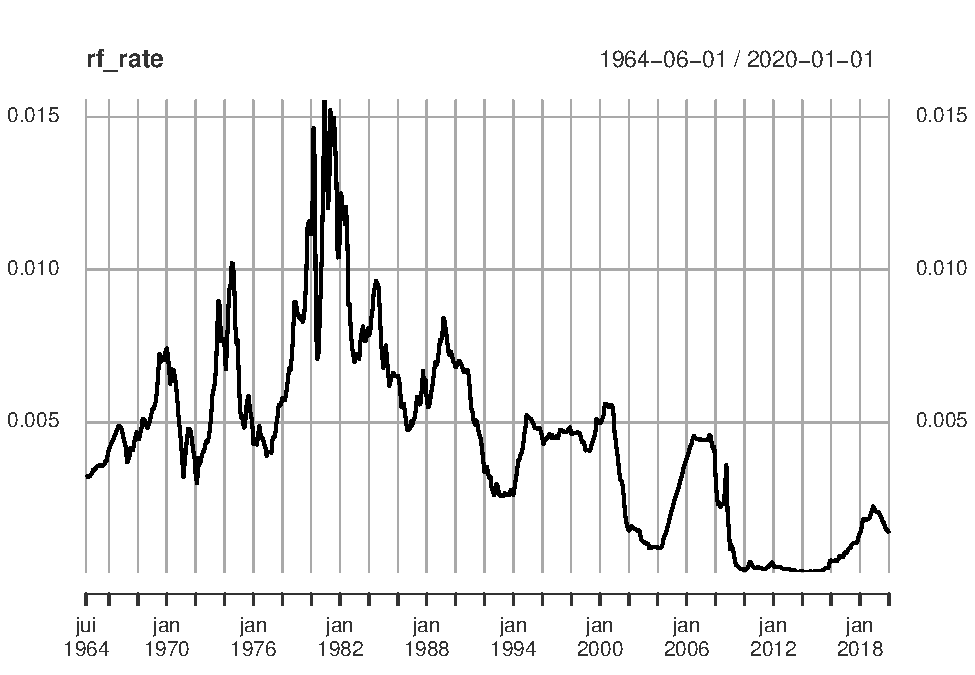
\includegraphics{TP-3_files/figure-latex/unnamed-chunk-5-1.pdf}
\caption{taux sans risque mensuel}
\end{figure}

\hypertarget{estimation-dun-moduxe8le-uxe0-un-facteur}{%
\section{Estimation d'un modèle à un
facteur}\label{estimation-dun-moduxe8le-uxe0-un-facteur}}

\begin{itemize}
\tightlist
\item
  Utiliser l'indice SPY comme proxy pour le marché et estimer pour
  chaque titre le modèle:
\end{itemize}

\[
R_i(t) - R_f(t) = \alpha + \beta (R_M(t) - R_f(t)) + \epsilon(t)
\] en utilisant la fonction \texttt{lm}.

\begin{itemize}
\tightlist
\item
  Placer chaque titre sur un diagramme rendement/beta et calculer par
  regression la droite de marché des titres risqués.
\end{itemize}

\begin{Shaded}
\begin{Highlighting}[]
\NormalTok{assets }\OtherTok{\textless{}{-}} \FunctionTok{names}\NormalTok{(monthly.ret)[}\FunctionTok{names}\NormalTok{(monthly.ret) }\SpecialCharTok{!=} \StringTok{"SPY"}\NormalTok{]}
\NormalTok{get.ret.beta }\OtherTok{\textless{}{-}} \ControlFlowTok{function}\NormalTok{(ret)\{}
\NormalTok{  res.mean }\OtherTok{\textless{}{-}} \FunctionTok{apply}\NormalTok{(ret,}\DecValTok{2}\NormalTok{,mean)}
\NormalTok{  res.mean }\OtherTok{\textless{}{-}}\NormalTok{ res.mean }\SpecialCharTok{{-}} \FunctionTok{mean}\NormalTok{(rf\_rate)}
\NormalTok{  res.mean }\OtherTok{\textless{}{-}}\NormalTok{ res.mean[assets]}

\NormalTok{  ret.minus.rf }\OtherTok{\textless{}{-}} \FunctionTok{as.data.frame}\NormalTok{(}\FunctionTok{lapply}\NormalTok{(ret, }\ControlFlowTok{function}\NormalTok{(col) col}\SpecialCharTok{{-}}\NormalTok{ret}\SpecialCharTok{$}\NormalTok{Rf))}
\NormalTok{  ret.minus.rf }\OtherTok{\textless{}{-}}\NormalTok{ ret.minus.rf[}\FunctionTok{names}\NormalTok{(ret.minus.rf) }\SpecialCharTok{!=} \StringTok{"Rf"}\NormalTok{]}

\NormalTok{  model }\OtherTok{\textless{}{-}} \FunctionTok{lapply}\NormalTok{(ret.minus.rf, }\ControlFlowTok{function}\NormalTok{(col) }\FunctionTok{lm}\NormalTok{(col }\SpecialCharTok{\textasciitilde{}}\NormalTok{ ret.minus.rf}\SpecialCharTok{$}\NormalTok{SPY))}

\NormalTok{  res.beta }\OtherTok{\textless{}{-}} \FunctionTok{lapply}\NormalTok{(model, }\ControlFlowTok{function}\NormalTok{(value) }\FunctionTok{coefficients}\NormalTok{(value)[}\DecValTok{2}\NormalTok{])}
\NormalTok{  res.beta }\OtherTok{\textless{}{-}}\NormalTok{ res.beta[}\FunctionTok{names}\NormalTok{(res.beta) }\SpecialCharTok{!=} \StringTok{"SPY"}\NormalTok{]}

  \FunctionTok{return}\NormalTok{(}\FunctionTok{as.data.frame}\NormalTok{(}\FunctionTok{cbind}\NormalTok{(res.mean,res.beta)))}

\NormalTok{\}}
\NormalTok{ret.beta.all }\OtherTok{\textless{}{-}} \FunctionTok{get.ret.beta}\NormalTok{(monthly.ret}\FloatTok{.2}\NormalTok{)}
\end{Highlighting}
\end{Shaded}

\begin{figure}
\centering
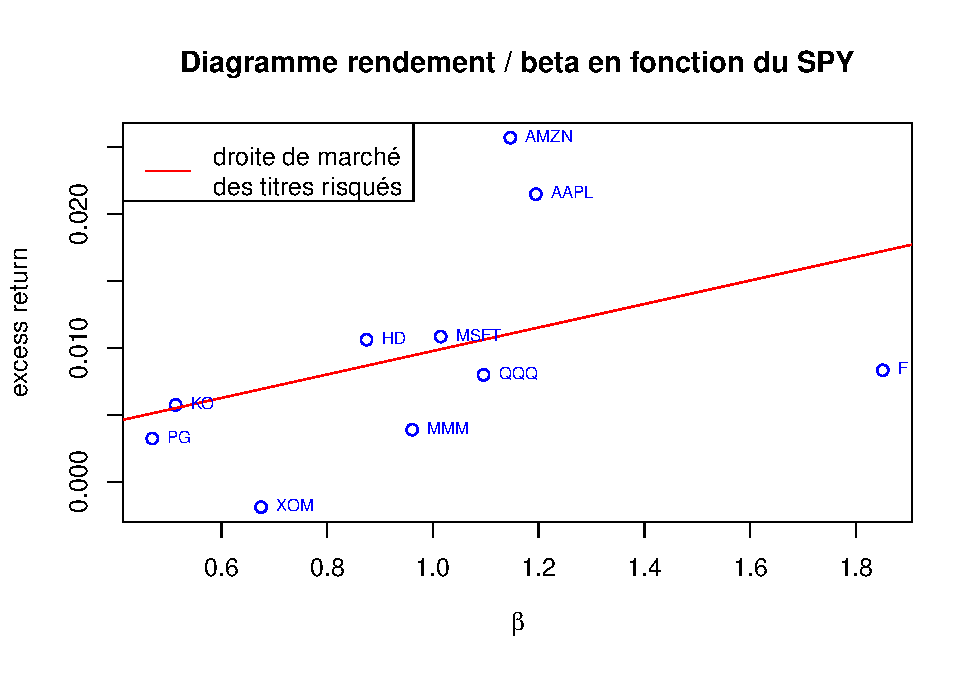
\includegraphics{TP-3_files/figure-latex/fig-1-1.pdf}
\caption{diagramme rendement béta de chaque titre}
\end{figure}

\begin{itemize}
\tightlist
\item
  En déduire les titres qui, selon ce modèle, \emph{semblent} chers et
  ceux qui semblent sous-évalués.
\end{itemize}

Les titres se trouvant au-dessus de la droite de marché sont considérés
comme sous-évalués tandis que les titres se trouvant en-dessous sont
surévalués. Certains titres ne sont pas exactement sur cette droite,
cependant ils ne s'en éloignent pas trop. On peut dire que :

\textbf{sous-évalués :}

\begin{itemize}
\tightlist
\item
  Apple (AAPL)
\item
  Amazon (AMZN)
\end{itemize}

\textbf{surévalués :}

\begin{itemize}
\tightlist
\item
  XOM
\item
  MMM
\item
  F
\end{itemize}

Est-ce que ces mesures de cherté relative vous semble correctes? Essayez
de mesurer la robustesse de ce calcul en estimant le modèles sur des
sous-intervalles de temps.

Présentez vos résultats de manière synthétique.

Dans un premier temps, nous avons réalisé la même modélisation pour
chaque année.\\
Au lieu d'appliquer la regression sur toutes les données, nous les avons
appliquer distinctement pour chaque année.

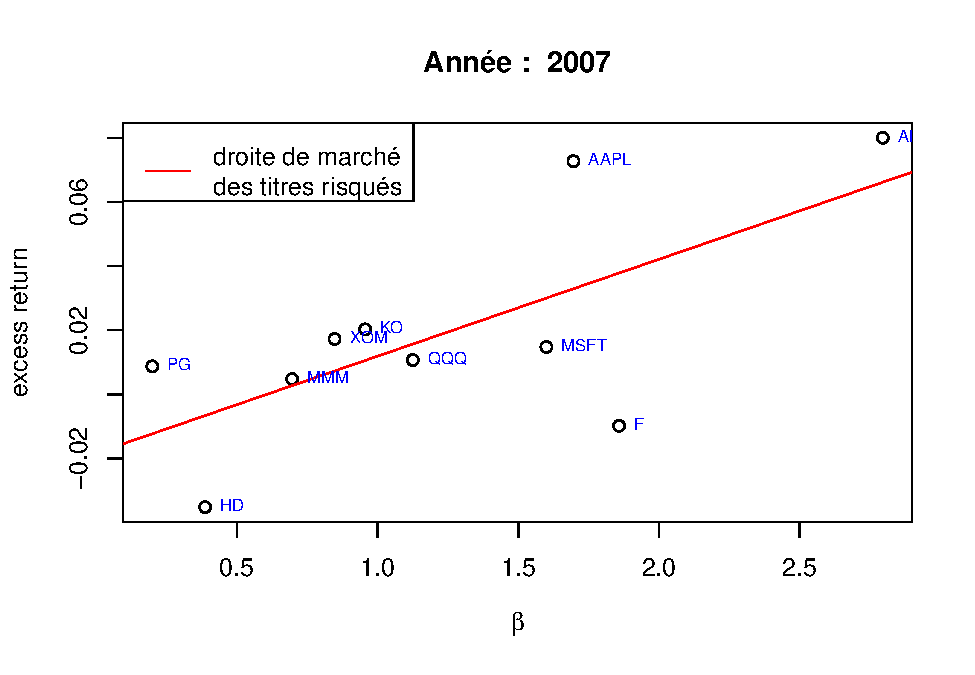
\includegraphics[width=0.5\linewidth,height=0.5\textheight]{TP-3_files/figure-latex/fig-2-1}
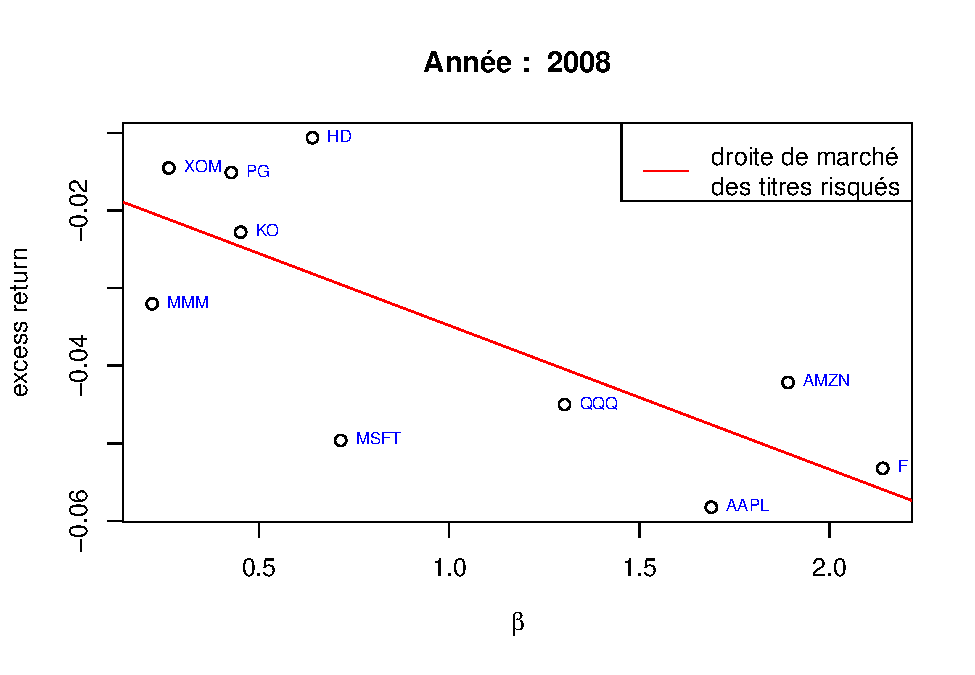
\includegraphics[width=0.5\linewidth,height=0.5\textheight]{TP-3_files/figure-latex/fig-2-2}
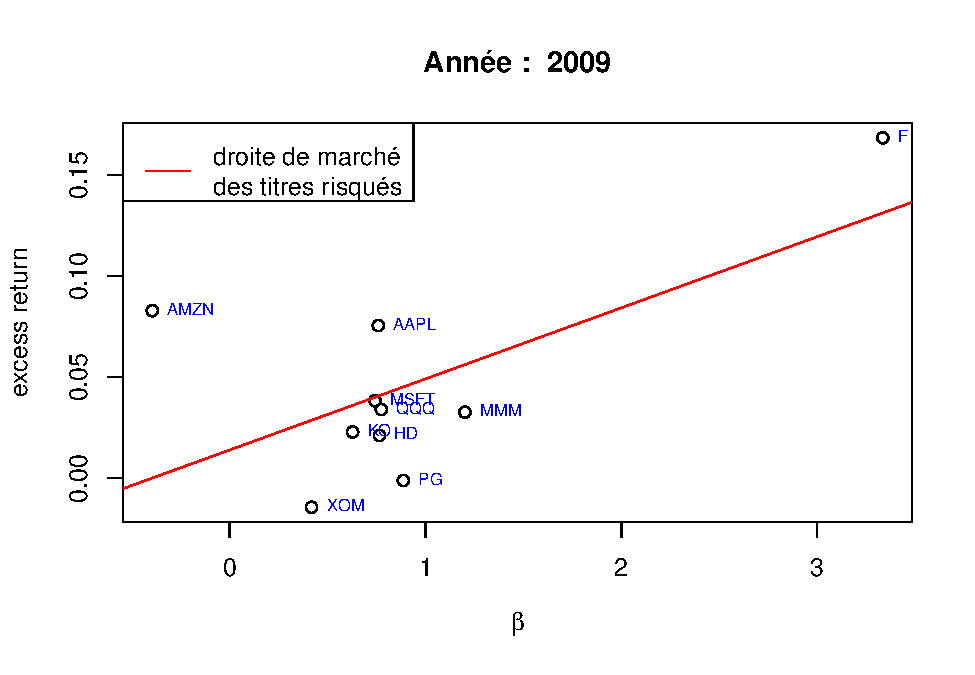
\includegraphics[width=0.5\linewidth,height=0.5\textheight]{TP-3_files/figure-latex/fig-2-3}
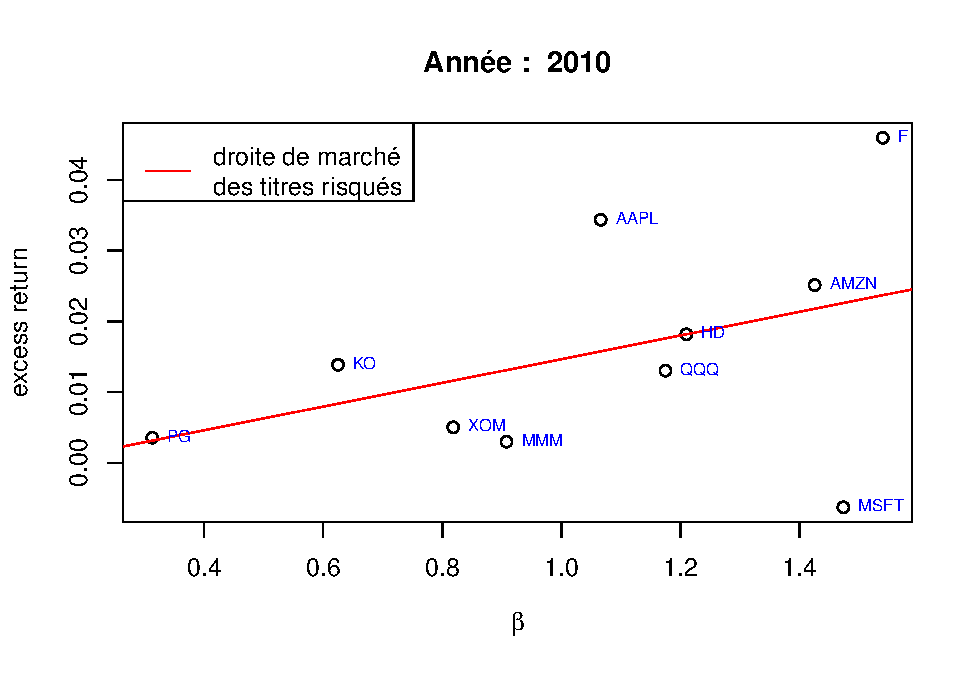
\includegraphics[width=0.5\linewidth,height=0.5\textheight]{TP-3_files/figure-latex/fig-2-4}
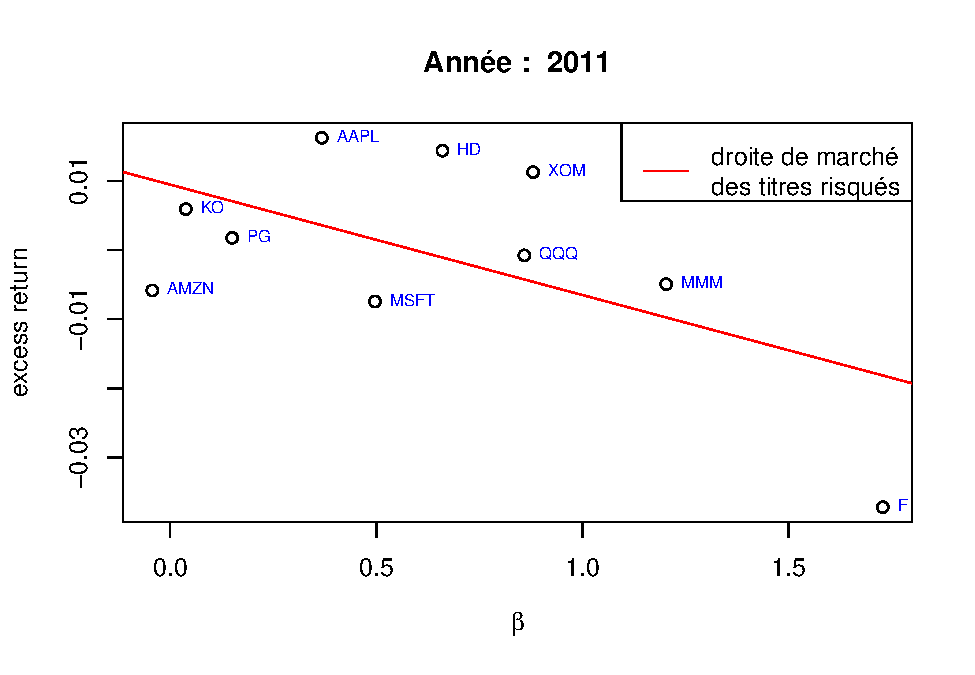
\includegraphics[width=0.5\linewidth,height=0.5\textheight]{TP-3_files/figure-latex/fig-2-5}
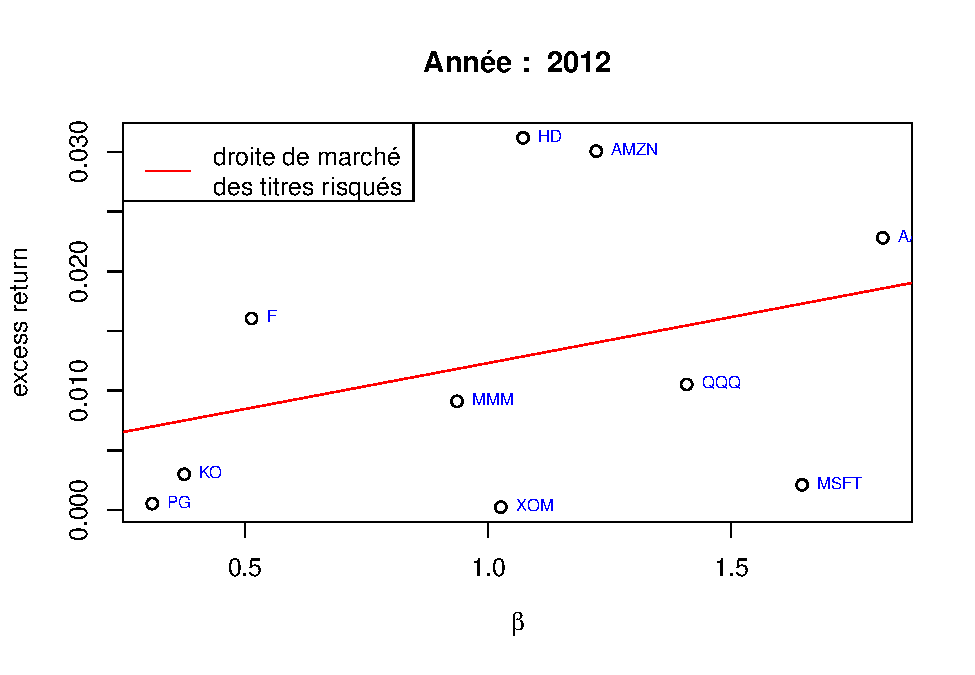
\includegraphics[width=0.5\linewidth,height=0.5\textheight]{TP-3_files/figure-latex/fig-2-6}
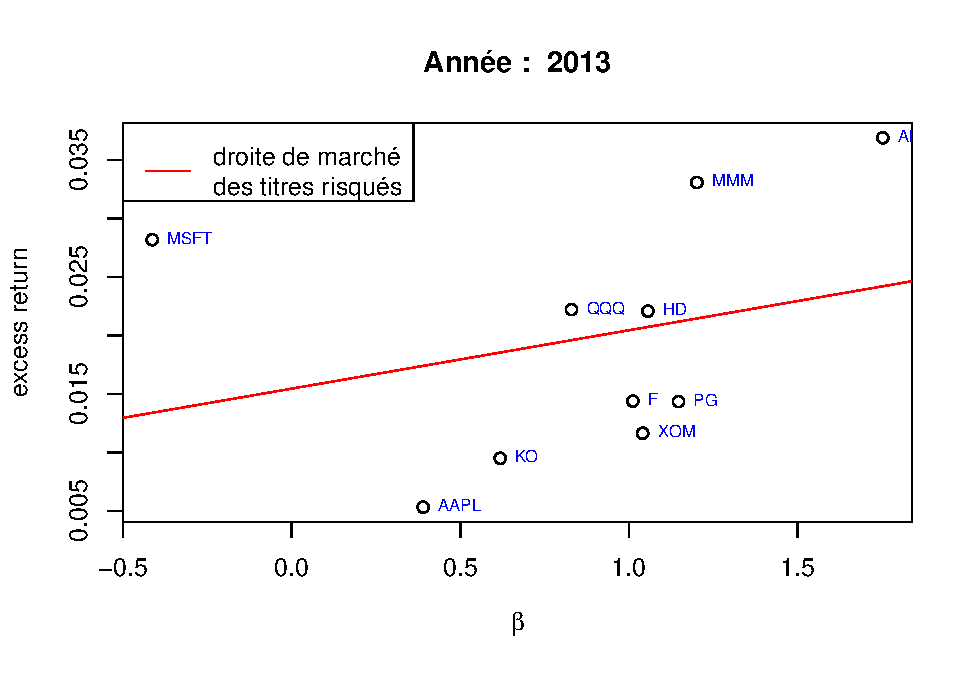
\includegraphics[width=0.5\linewidth,height=0.5\textheight]{TP-3_files/figure-latex/fig-2-7}
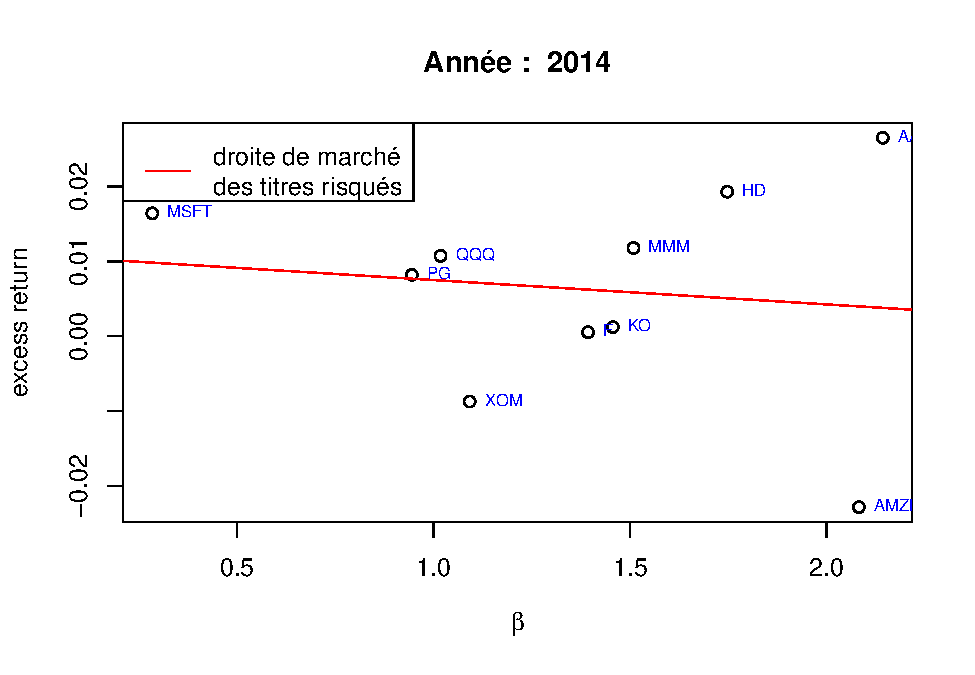
\includegraphics[width=0.5\linewidth,height=0.5\textheight]{TP-3_files/figure-latex/fig-2-8}
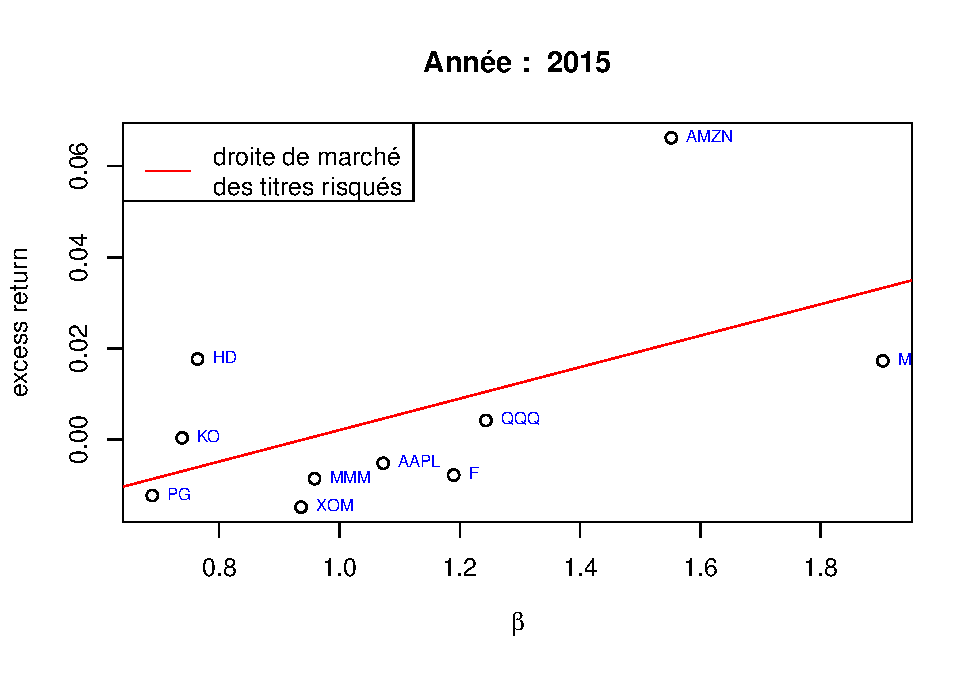
\includegraphics[width=0.5\linewidth,height=0.5\textheight]{TP-3_files/figure-latex/fig-2-9}
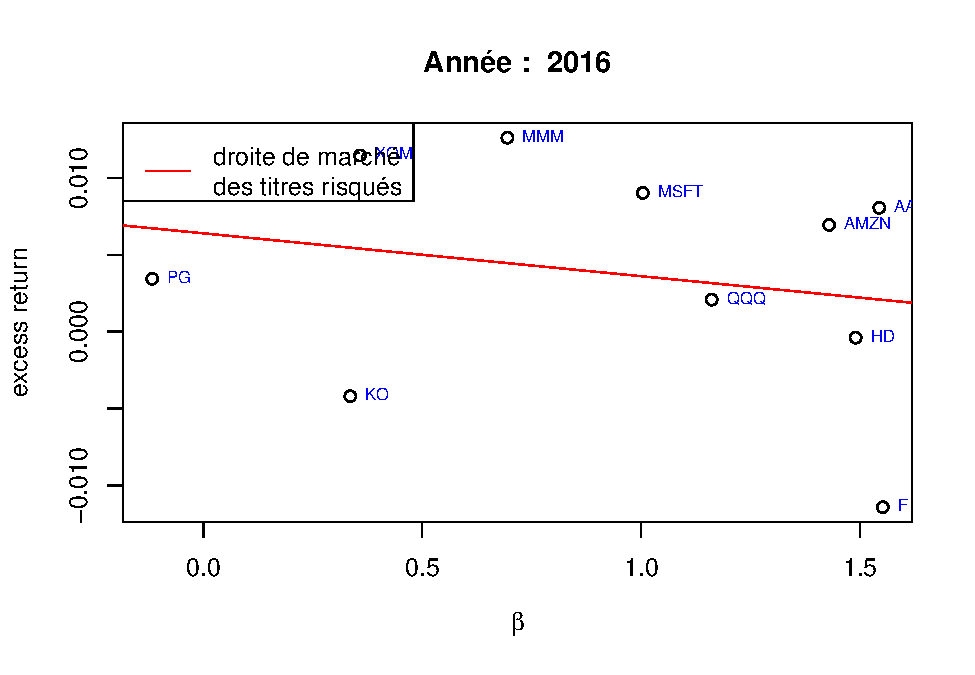
\includegraphics[width=0.5\linewidth,height=0.5\textheight]{TP-3_files/figure-latex/fig-2-10}
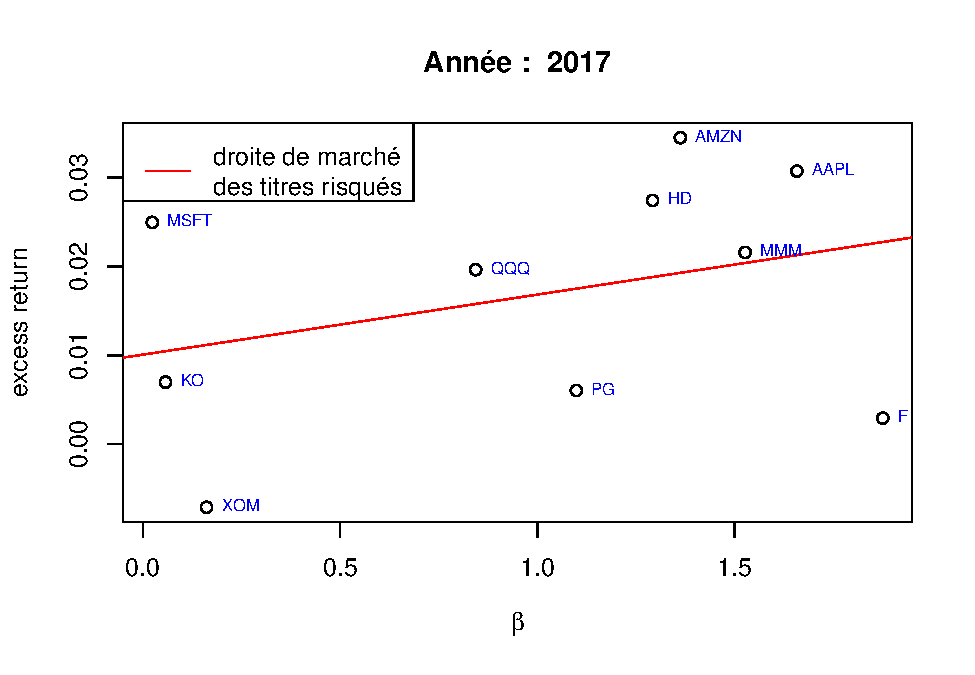
\includegraphics[width=0.5\linewidth,height=0.5\textheight]{TP-3_files/figure-latex/fig-2-11}
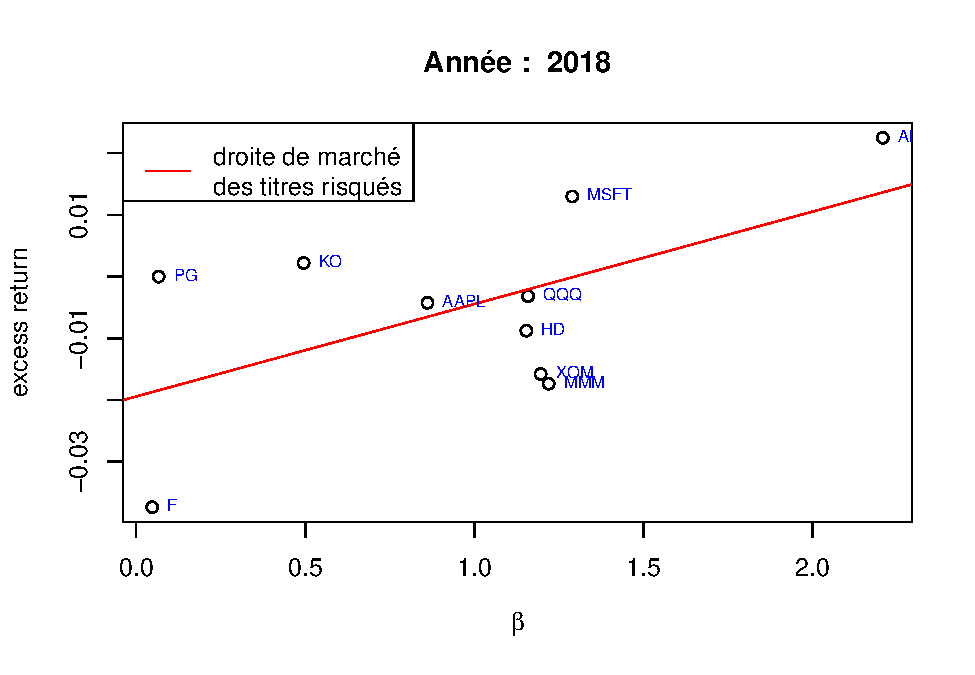
\includegraphics[width=0.5\linewidth,height=0.5\textheight]{TP-3_files/figure-latex/fig-2-12}
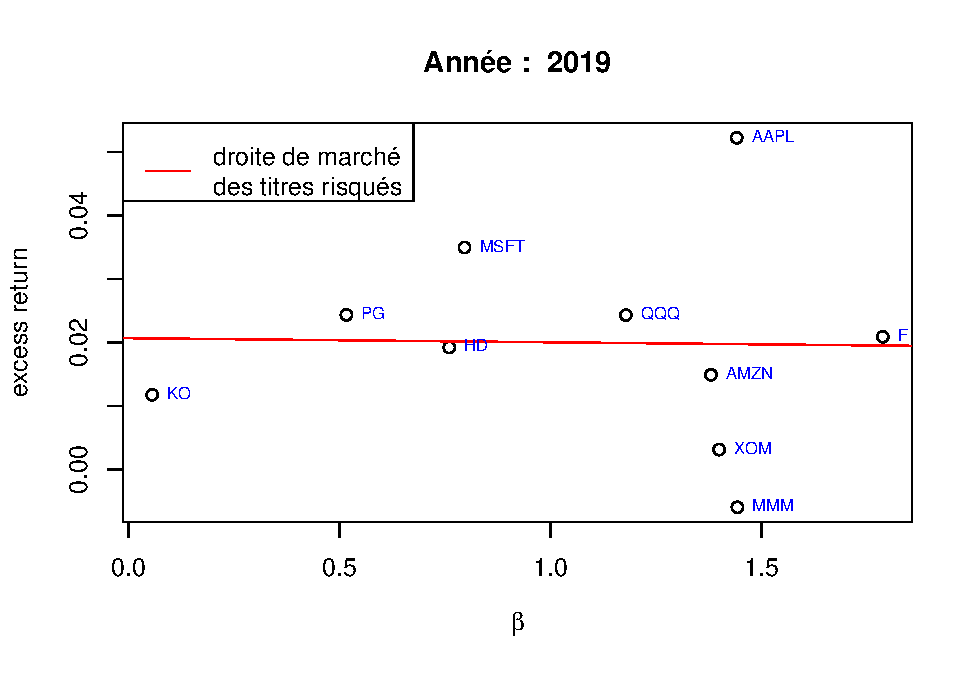
\includegraphics[width=0.5\linewidth,height=0.5\textheight]{TP-3_files/figure-latex/fig-2-13}

Nous avons tracé les diagrammes rendement / béta pour chaque année entre
2007 et 2020. On peut remarquer que Apple est sous-évalué dans les
années 2007, 2009, 2010 alors qu'il est surévalué dans les années 2008,
2013, 2015. Ceci est un exemple mais on pourrait faire la même remarque
pour chaque titre. Ceci nous ammène à remmettre en cause la robustesse
de cette méthode. En effet selon les intervalles de temps nous obtenons
des résultats contradictoires.

\begin{Shaded}
\begin{Highlighting}[]
\NormalTok{names\_ }\OtherTok{\textless{}{-}} \FunctionTok{names}\NormalTok{(}\FunctionTok{get.ret.beta}\NormalTok{(monthly.ret}\FloatTok{.2}\NormalTok{)}\SpecialCharTok{$}\NormalTok{res.mean)}
\NormalTok{beta.roll }\OtherTok{\textless{}{-}} \FunctionTok{na.omit}\NormalTok{(}\FunctionTok{rollapply}\NormalTok{(}
  \AttributeTok{data=}\NormalTok{monthly.ret}\FloatTok{.2}\NormalTok{,}
  \AttributeTok{FUN=}\ControlFlowTok{function}\NormalTok{(data) }\FunctionTok{as.numeric}\NormalTok{(}\FunctionTok{get.ret.beta}\NormalTok{(data)}\SpecialCharTok{$}\NormalTok{res.beta),}
  \AttributeTok{width=}\DecValTok{36}\NormalTok{,}
  \AttributeTok{by.column=}\ConstantTok{FALSE}\NormalTok{))}
\NormalTok{alpha.roll }\OtherTok{\textless{}{-}} \FunctionTok{na.omit}\NormalTok{(}\FunctionTok{rollapply}\NormalTok{(}
  \AttributeTok{data=}\NormalTok{monthly.ret}\FloatTok{.2}\NormalTok{,}
  \AttributeTok{FUN=}\ControlFlowTok{function}\NormalTok{(data) }\FunctionTok{as.numeric}\NormalTok{(}\FunctionTok{get.ret.beta}\NormalTok{(data)}\SpecialCharTok{$}\NormalTok{res.mean),}
  \AttributeTok{width=}\DecValTok{36}\NormalTok{,}
  \AttributeTok{by.column=}\ConstantTok{FALSE}\NormalTok{))}
\FunctionTok{names}\NormalTok{(beta.roll) }\OtherTok{\textless{}{-}}\NormalTok{ names\_}
\FunctionTok{names}\NormalTok{(alpha.roll) }\OtherTok{\textless{}{-}}\NormalTok{ names\_}
\end{Highlighting}
\end{Shaded}

\begin{figure}
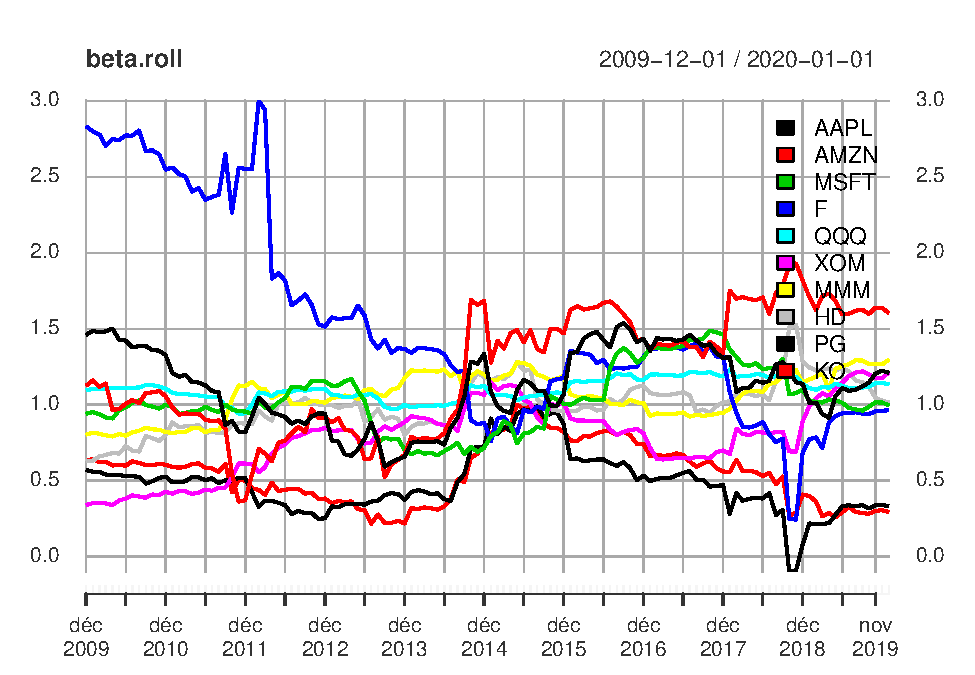
\includegraphics[width=0.5\linewidth]{TP-3_files/figure-latex/fig-3-1} 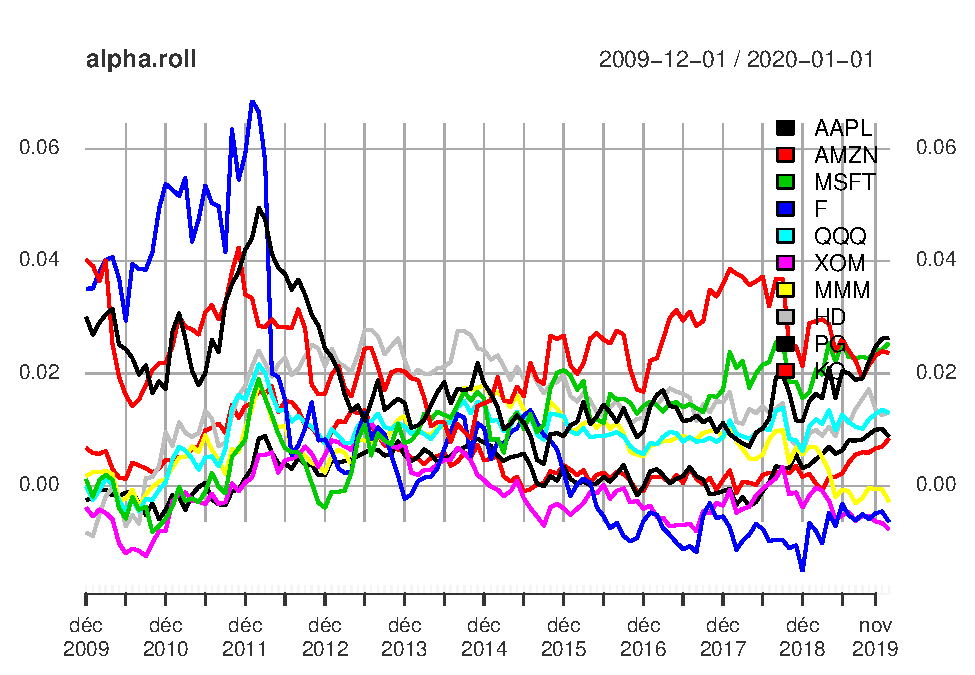
\includegraphics[width=0.5\linewidth]{TP-3_files/figure-latex/fig-3-2} \caption{rolling beta / alpha }\label{fig:fig-3}
\end{figure}

Afin d'avoir une analyse plus précise, nous avons calculé les \(\beta\)
et \(\alpha\) pour chaque titre sur des fenêtres glissantes (de taille
36). On remarque que les \(\beta\) varient dans un ``range'' assez
important alors que les variations des \(\alpha\) sont moins
importantes.

Le modèle utilisé montre des limites pour l'estimation des \(\beta\)

\hypertarget{moduxe8le-de-treynor-black}{%
\section{Modèle de Treynor-Black}\label{moduxe8le-de-treynor-black}}

Le modèle de Treynor-Black a pour objectif d'exploiter les informations
calculées en première partie. L'idée étant de constituer un portefeuille
``actif'' avec les titres qui semblent mal valorisés par le marché, et
allouer le reste de sa richesse au portefeuille de marché.

\hypertarget{selection-des-titres-uxe0-inclure-dans-le-portefeuille-actif.}{%
\subsection{Selection des titres à inclure dans le portefeuille
actif.}\label{selection-des-titres-uxe0-inclure-dans-le-portefeuille-actif.}}

C'est l'étape délicate de la méthode de Treynor-Black. A partir de
l'évaluation du modèle à un facteur, déterminez quels titres méritent de
figurer dans le portefeuille actif. En théorie, on a envie d'acheter les
titres sous-cotés (\(\alpha_i > 0\)) mais cette anomalie n'est peut être
qu'apparente! Il faut également apprécier la qualité de l'estimation
statistique.

En testant diverses combinaisons de titres à mettre dans le portefeuille
actif, vous pourrez mesurer la sensibilité de modèle de Treynor-Black
aux données.

\begin{Shaded}
\begin{Highlighting}[]
\NormalTok{monthly.ret.minus.rf }\OtherTok{\textless{}{-}} \FunctionTok{as.data.frame}\NormalTok{(monthly.ret }\SpecialCharTok{{-}} \FunctionTok{mean}\NormalTok{(rf\_rate))}
\NormalTok{model }\OtherTok{\textless{}{-}} \FunctionTok{lapply}\NormalTok{(monthly.ret.minus.rf, }\ControlFlowTok{function}\NormalTok{(col) }\FunctionTok{lm}\NormalTok{(col }\SpecialCharTok{\textasciitilde{}}\NormalTok{ monthly.ret.minus.rf}\SpecialCharTok{$}\NormalTok{SPY))}
\NormalTok{model }\OtherTok{\textless{}{-}}\NormalTok{ model[}\FunctionTok{names}\NormalTok{(model) }\SpecialCharTok{!=} \StringTok{"SPY"}\NormalTok{]}
\end{Highlighting}
\end{Shaded}

\begin{itemize}
\tightlist
\item
  Sélectionner les \(\alpha_{i} > 0\)
\end{itemize}

\begin{Shaded}
\begin{Highlighting}[]
\NormalTok{titre.selected.simple }\OtherTok{\textless{}{-}} \FunctionTok{names}\NormalTok{(}
\NormalTok{  model[}\FunctionTok{lapply}\NormalTok{(model, }\ControlFlowTok{function}\NormalTok{(titre) }\FunctionTok{coefficients}\NormalTok{(titre)[}\DecValTok{1}\NormalTok{]) }
  \SpecialCharTok{\textgreater{}} \DecValTok{0}\NormalTok{]}
\NormalTok{  )}
\end{Highlighting}
\end{Shaded}

\begin{verbatim}
## [1] "AAPL" "AMZN" "MSFT" "F"    "QQQ"  "MMM"  "HD"   "PG"   "KO"
\end{verbatim}

\begin{itemize}
\tightlist
\item
  Test statistique, niveau de confiance à 95\% / 99\% \(\alpha_{i} > 0\)
\end{itemize}

\begin{Shaded}
\begin{Highlighting}[]
\NormalTok{titre.selected.inter }\OtherTok{\textless{}{-}} \FunctionTok{names}\NormalTok{(}
\NormalTok{  model[}\FunctionTok{as.logical}\NormalTok{(}\FunctionTok{lapply}\NormalTok{(model,}
  \ControlFlowTok{function}\NormalTok{(titre) }\FunctionTok{confint}\NormalTok{(titre)[}\DecValTok{1}\NormalTok{,}\DecValTok{1}\NormalTok{]}\SpecialCharTok{\textgreater{}}\DecValTok{0} \SpecialCharTok{\&} \FunctionTok{confint}\NormalTok{(titre)[}\DecValTok{1}\NormalTok{,}\DecValTok{2}\NormalTok{]}\SpecialCharTok{\textgreater{}}\DecValTok{0}\NormalTok{))]}
\NormalTok{  )}
\end{Highlighting}
\end{Shaded}

\begin{verbatim}
## [1] "AAPL" "AMZN" "QQQ"  "HD"
\end{verbatim}

\hypertarget{duxe9termination-du-portefeuille-actif}{%
\subsection{Détermination du portefeuille
actif}\label{duxe9termination-du-portefeuille-actif}}

Ayant choisi les titres à inclure dans le portefeuille actif, on
rappelle que le poids de chaque titre dans le portefeuille actif est
proportionnel au ratio \(\alpha_i/\sigma^2(\epsilon_i)\):

\[
w_i = \frac{\alpha_i/\sigma^2(\epsilon_i)}{\sum_i \alpha_i/\sigma^2(\epsilon_i)}
\]

Calculer les poids des actifs dans le portefeuille actif. Justifier
votre choix d'inclure ou d'exclure tel ou tel instrument.

\begin{Shaded}
\begin{Highlighting}[]
\NormalTok{get.weight }\OtherTok{\textless{}{-}} \ControlFlowTok{function}\NormalTok{(model) \{}
\NormalTok{  alpha }\OtherTok{\textless{}{-}} \FunctionTok{as.data.frame}\NormalTok{(}\FunctionTok{lapply}\NormalTok{(model, }\ControlFlowTok{function}\NormalTok{(model) \{}\FunctionTok{coefficients}\NormalTok{(model)[}\DecValTok{1}\NormalTok{]\}))}
\NormalTok{  residual }\OtherTok{\textless{}{-}} \FunctionTok{as.data.frame}\NormalTok{(}\FunctionTok{lapply}\NormalTok{(model, }\ControlFlowTok{function}\NormalTok{(model) \{}\FunctionTok{sigma}\NormalTok{(model)\}))}
\NormalTok{  denominateur }\OtherTok{\textless{}{-}} \FunctionTok{sum}\NormalTok{(alpha }\SpecialCharTok{/}\NormalTok{ residual)}
  \FunctionTok{return}\NormalTok{(alpha }\SpecialCharTok{/}\NormalTok{ residual }\SpecialCharTok{/}\NormalTok{ denominateur)}

\NormalTok{\}}
\NormalTok{simple.weight }\OtherTok{\textless{}{-}} \FunctionTok{get.weight}\NormalTok{(model[}\FunctionTok{names}\NormalTok{(model) }\SpecialCharTok{\%in\%}\NormalTok{ titre.selected.simple])}
\NormalTok{inter.weight }\OtherTok{\textless{}{-}} \FunctionTok{get.weight}\NormalTok{(model[}\FunctionTok{names}\NormalTok{(model) }\SpecialCharTok{\%in\%}\NormalTok{ titre.selected.inter])}
\end{Highlighting}
\end{Shaded}

\begin{table}[H]

\caption{\label{tab:unnamed-chunk-14}Poids (hypothèse simple)}
\centering
\begin{tabular}[t]{rrrrrrrrr}
\toprule
AAPL & AMZN & MSFT & F & QQQ & MMM & HD & PG & KO\\
\midrule
0.201 & 0.215 & 0.124 & 0.008 & 0.184 & 0.01 & 0.138 & 0.033 & 0.088\\
\bottomrule
\end{tabular}
\end{table}

\begin{table}[H]

\caption{\label{tab:unnamed-chunk-14}Poids (interval confiance)}
\centering
\begin{tabular}[t]{rrrr}
\toprule
AAPL & AMZN & QQQ & HD\\
\midrule
0.272 & 0.292 & 0.249 & 0.187\\
\bottomrule
\end{tabular}
\end{table}

Calculez les valeurs suivantes concernant le portefeuille actif:

\begin{description}
\item[$R_A$] Excess de rendement
\item[$\alpha_A$] alpha du portefeuille actif
\item[$\beta_A$]  beta du portefeuille actif
\item[$\sigma_A$] ecart-type du portefeuille actif
\item[$\sigma^2(e_A)$] variance résiduelle du portefeuille actif

\end{description}

\begin{table}[H]

\caption{\label{tab:unnamed-chunk-16}Résumé des portefeuilles}
\centering
\begin{tabular}[t]{lrr}
\toprule
  & simple & interval\\
\midrule
R\_a & 0.0191259 & 0.0219396\\
alpha\_a & 0.0113812 & 0.0136032\\
beta\_a & 1.0209686 & 1.0989694\\
sigma\_a & 0.1076089 & 0.1338812\\
sigma2\_ea & 0.0097504 & 0.0158047\\
\bottomrule
\end{tabular}
\end{table}

\hypertarget{duxe9termination-de-la-ponduxe9ration-entre-le-portefeuille-actif-et-le-portefeuille-de-marchuxe9.}{%
\subsection{Détermination de la pondération entre le portefeuille actif
et le portefeuille de
marché.}\label{duxe9termination-de-la-ponduxe9ration-entre-le-portefeuille-actif-et-le-portefeuille-de-marchuxe9.}}

On rappelle l'allocation de richesse au portefeuille actif:

\[
w_A = \frac{\alpha_A \sigma^2_M}{\alpha_A \sigma^2_M (1-\beta_A) + R_M \sigma^2(e_A)}
\]

Avec:

\[
\begin{aligned}
R_A & = \alpha_A + \beta_A R_M \\
\sigma^2_A & = \beta^2_A \sigma^2_M + \sigma^2(e_A)
\end{aligned}
\]

\hypertarget{capital-allocation-line}{%
\subsection{Capital Allocation Line}\label{capital-allocation-line}}

Calculez l'espérance de rendement et le risque de quelques portefeuilles
situés sur la ``Capital Allocation Line'' qui joint l'actif sans risque
et le portefeuille tangent. Placez la solution du modèle de
Treynor-Black, le portefeuille actif et le portefeuille de marché sur le
graphique ci-dessous.

\begin{Shaded}
\begin{Highlighting}[]
\NormalTok{Assets }\OtherTok{\textless{}{-}} \FunctionTok{c}\NormalTok{(}\StringTok{"AAPL"}\NormalTok{, }\StringTok{"AMZN"}\NormalTok{, }\StringTok{"MSFT"}\NormalTok{, }\StringTok{"F"}\NormalTok{,  }\StringTok{"XOM"}\NormalTok{, }\StringTok{"MMM"}\NormalTok{,  }\StringTok{"HD"}\NormalTok{,   }\StringTok{"PG"}\NormalTok{,   }\StringTok{"KO"}\NormalTok{)}
\NormalTok{plot.data }\OtherTok{\textless{}{-}}\NormalTok{ monthly.ret}\FloatTok{.2}\NormalTok{[, }\FunctionTok{c}\NormalTok{(Assets, }\StringTok{"Rf"}\NormalTok{)]}
\ControlFlowTok{for}\NormalTok{(a }\ControlFlowTok{in}\NormalTok{ Assets) \{}
\NormalTok{  plot.data[, a] }\OtherTok{\textless{}{-}}\NormalTok{ plot.data[, a] }\SpecialCharTok{{-}}\NormalTok{ plot.data}\SpecialCharTok{$}\NormalTok{Rf}
\NormalTok{  \}}

\NormalTok{res }\OtherTok{\textless{}{-}} \FunctionTok{data.frame}\NormalTok{(}\AttributeTok{Mean=}\FunctionTok{apply}\NormalTok{(plot.data[, Assets],}\DecValTok{2}\NormalTok{,mean),}
                  \AttributeTok{Sd =} \FunctionTok{apply}\NormalTok{(plot.data[, Assets],}\DecValTok{2}\NormalTok{,sd))}
\FunctionTok{rownames}\NormalTok{(res) }\OtherTok{\textless{}{-}}\NormalTok{ Assets}
\end{Highlighting}
\end{Shaded}

\begin{Shaded}
\begin{Highlighting}[]
\CommentTok{\# Capital Market line}
\NormalTok{mu }\OtherTok{\textless{}{-}} \FunctionTok{colMeans}\NormalTok{(monthly.ret[,Assets])}
\NormalTok{mu.free }\OtherTok{\textless{}{-}} \FunctionTok{mean}\NormalTok{(rf\_rate)}
\NormalTok{mu.star.v }\OtherTok{\textless{}{-}} \FunctionTok{seq}\NormalTok{(}\AttributeTok{from=}\NormalTok{mu.free,}\AttributeTok{to=}\FloatTok{0.35}\NormalTok{,}\AttributeTok{length.out=}\DecValTok{30}\NormalTok{)}
\NormalTok{n }\OtherTok{\textless{}{-}} \FunctionTok{length}\NormalTok{(mu)}
\NormalTok{Sigma }\OtherTok{\textless{}{-}} \FunctionTok{cov}\NormalTok{(monthly.ret[,Assets])}

\NormalTok{optim.with.rf }\OtherTok{\textless{}{-}} \ControlFlowTok{function}\NormalTok{(mu.star)\{}
\NormalTok{  A.sum }\OtherTok{\textless{}{-}} \FunctionTok{matrix}\NormalTok{(mu }\SpecialCharTok{{-}}\NormalTok{ mu.free, }\AttributeTok{ncol=}\DecValTok{1}\NormalTok{)}
\NormalTok{  A.mat }\OtherTok{\textless{}{-}} \FunctionTok{cbind}\NormalTok{(A.sum,}\FunctionTok{rep}\NormalTok{(}\DecValTok{1}\NormalTok{,n))}
\NormalTok{  b }\OtherTok{\textless{}{-}} \FunctionTok{c}\NormalTok{(mu.star,}\DecValTok{1}\NormalTok{)}
  \FunctionTok{return}\NormalTok{(}\FunctionTok{solve.QP}\NormalTok{(}\DecValTok{2}\SpecialCharTok{*}\NormalTok{Sigma, }\FunctionTok{rep}\NormalTok{(}\DecValTok{0}\NormalTok{,n),A.mat,b,}\AttributeTok{meq=}\DecValTok{2}\NormalTok{))}
\NormalTok{\}}

\NormalTok{sol.with.rf }\OtherTok{\textless{}{-}} \ConstantTok{NULL}
\ControlFlowTok{for}\NormalTok{(mu.star }\ControlFlowTok{in}\NormalTok{ mu.star.v) \{}
\NormalTok{  qp }\OtherTok{\textless{}{-}} \FunctionTok{optim.with.rf}\NormalTok{(mu.star)}

\NormalTok{  tmp }\OtherTok{\textless{}{-}} \FunctionTok{matrix}\NormalTok{(}\FunctionTok{c}\NormalTok{(mu.star,}\FunctionTok{sqrt}\NormalTok{(qp}\SpecialCharTok{$}\NormalTok{value)),}\AttributeTok{nrow=}\DecValTok{1}\NormalTok{)}

  \ControlFlowTok{if}\NormalTok{(}\FunctionTok{is.null}\NormalTok{(sol.with.rf))\{}
\NormalTok{    sol.with.rf }\OtherTok{\textless{}{-}}\NormalTok{ tmp}
\NormalTok{  \} }\ControlFlowTok{else}\NormalTok{\{}
\NormalTok{    sol.with.rf }\OtherTok{\textless{}{-}} \FunctionTok{rbind}\NormalTok{(sol.with.rf,tmp)}
\NormalTok{  \}}
\NormalTok{\}}
\end{Highlighting}
\end{Shaded}

\begin{Shaded}
\begin{Highlighting}[]
\CommentTok{\# market portfolio}
\NormalTok{mu }\OtherTok{\textless{}{-}} \FunctionTok{colMeans}\NormalTok{(monthly.ret}\FloatTok{.2}\NormalTok{)}
\NormalTok{sig2 }\OtherTok{\textless{}{-}} \FunctionTok{cov}\NormalTok{(monthly.ret[,Assets])}

\NormalTok{w.t.nom }\OtherTok{\textless{}{-}} \FunctionTok{solve}\NormalTok{(sig2,mu[Assets] }\SpecialCharTok{{-}}\NormalTok{ mu[}\StringTok{"Rf"}\NormalTok{])}
\NormalTok{w.t.den }\OtherTok{\textless{}{-}} \FunctionTok{sum}\NormalTok{(w.t.nom)}
\NormalTok{w.t }\OtherTok{\textless{}{-}}\NormalTok{ w.t.nom }\SpecialCharTok{/}\NormalTok{ w.t.den}

\NormalTok{mu.t }\OtherTok{\textless{}{-}} \FunctionTok{t}\NormalTok{(mu[Assets] }\SpecialCharTok{{-}}\NormalTok{ mu.free) }\SpecialCharTok{\%*\%}\NormalTok{ w.t}
\NormalTok{sigma.t }\OtherTok{\textless{}{-}} \FunctionTok{sqrt}\NormalTok{(}\FunctionTok{t}\NormalTok{(w.t) }\SpecialCharTok{\%*\%}\NormalTok{ sig2 }\SpecialCharTok{\%*\%}\NormalTok{ w.t)}
\end{Highlighting}
\end{Shaded}

\begin{Shaded}
\begin{Highlighting}[]
\CommentTok{\# Active portfolio}
\NormalTok{get.active.port }\OtherTok{\textless{}{-}} \ControlFlowTok{function}\NormalTok{(weight)\{}
\NormalTok{  titres }\OtherTok{\textless{}{-}} \FunctionTok{names}\NormalTok{(weight)}
\NormalTok{  w.a }\OtherTok{\textless{}{-}} \FunctionTok{as.numeric}\NormalTok{(weight)}
\NormalTok{  sig2.a }\OtherTok{\textless{}{-}} \FunctionTok{cov}\NormalTok{(monthly.ret[,titres])}
\NormalTok{  mu.a }\OtherTok{\textless{}{-}} \FunctionTok{t}\NormalTok{(w.a) }\SpecialCharTok{\%*\%} \FunctionTok{as.numeric}\NormalTok{(}\FunctionTok{matrix}\NormalTok{(mu[titres]),}\AttributeTok{ncol=}\DecValTok{1}\NormalTok{)}
\NormalTok{  sigma.a }\OtherTok{\textless{}{-}} \FunctionTok{sqrt}\NormalTok{(}\FunctionTok{t}\NormalTok{(w.a) }\SpecialCharTok{\%*\%}\NormalTok{ sig2.a }\SpecialCharTok{\%*\%}\NormalTok{ w.a)}
  \FunctionTok{return}\NormalTok{(}\FunctionTok{data.frame}\NormalTok{(}\StringTok{"mu.a"} \OtherTok{=}\NormalTok{ mu.a,}\StringTok{"sigma.a"}\OtherTok{=}\NormalTok{sigma.a))}
\NormalTok{\}}
\NormalTok{active.inter }\OtherTok{\textless{}{-}} \FunctionTok{get.active.port}\NormalTok{(inter.weight)}
\NormalTok{active.simple }\OtherTok{\textless{}{-}} \FunctionTok{get.active.port}\NormalTok{(simple.weight)}
\end{Highlighting}
\end{Shaded}

\begin{Shaded}
\begin{Highlighting}[]
\CommentTok{\# Solution Treynor}
\NormalTok{get.w.A }\OtherTok{\textless{}{-}} \ControlFlowTok{function}\NormalTok{(port.summary)\{}
\NormalTok{  benchmark.var }\OtherTok{\textless{}{-}} \FunctionTok{var}\NormalTok{(monthly.ret}\SpecialCharTok{$}\NormalTok{SPY)}
\NormalTok{  benchmark.ret }\OtherTok{\textless{}{-}} \FunctionTok{mean}\NormalTok{(monthly.ret}\SpecialCharTok{$}\NormalTok{SPY)}
\NormalTok{  w.a.num }\OtherTok{\textless{}{-}}\NormalTok{ port.summary[}\StringTok{"alpha\_a"}\NormalTok{,] }\SpecialCharTok{*}\NormalTok{ benchmark.var}
\NormalTok{  w.a.den }\OtherTok{\textless{}{-}}\NormalTok{ port.summary[}\StringTok{"alpha\_a"}\NormalTok{,] }\SpecialCharTok{*}\NormalTok{ benchmark.var }\SpecialCharTok{*}\NormalTok{ (}\DecValTok{1} \SpecialCharTok{{-}}\NormalTok{ port.summary[}\StringTok{"beta\_a"}\NormalTok{,]) }\SpecialCharTok{+}\NormalTok{ benchmark.ret}\SpecialCharTok{*}\NormalTok{port.summary[}\StringTok{"sigma2\_ea"}\NormalTok{,]}
  \FunctionTok{return}\NormalTok{(w.a.num }\SpecialCharTok{/}\NormalTok{ w.a.den)}
\NormalTok{\}}
\NormalTok{get.TB.port }\OtherTok{\textless{}{-}} \ControlFlowTok{function}\NormalTok{(active.weight,active.port)\{}
\NormalTok{  w.TB }\OtherTok{=} \FunctionTok{c}\NormalTok{(active.weight,}\DecValTok{1}\SpecialCharTok{{-}}\NormalTok{active.weight)}
\NormalTok{  mu.TB }\OtherTok{\textless{}{-}} \FunctionTok{t}\NormalTok{(w.TB) }\SpecialCharTok{\%*\%} \FunctionTok{c}\NormalTok{(active.port}\SpecialCharTok{$}\NormalTok{mu.a,mu.t)}
\NormalTok{  sigma.TB }\OtherTok{=} \FunctionTok{t}\NormalTok{(w.TB) }\SpecialCharTok{\%*\%} \FunctionTok{c}\NormalTok{(active.port}\SpecialCharTok{$}\NormalTok{sigma.a,sigma.t)}
  \FunctionTok{return}\NormalTok{(}\FunctionTok{data.frame}\NormalTok{(}\StringTok{"mu.TB"}\OtherTok{=}\NormalTok{mu.TB,}\StringTok{"sigma.TB"}\OtherTok{=}\NormalTok{sigma.TB))}
\NormalTok{\}}

\NormalTok{TB.inter }\OtherTok{\textless{}{-}} \FunctionTok{get.TB.port}\NormalTok{(}\FunctionTok{get.w.A}\NormalTok{(inter.summary),active.inter)}
\NormalTok{TB.simple }\OtherTok{\textless{}{-}} \FunctionTok{get.TB.port}\NormalTok{(}\FunctionTok{get.w.A}\NormalTok{(simple.summary),active.simple)}
\end{Highlighting}
\end{Shaded}

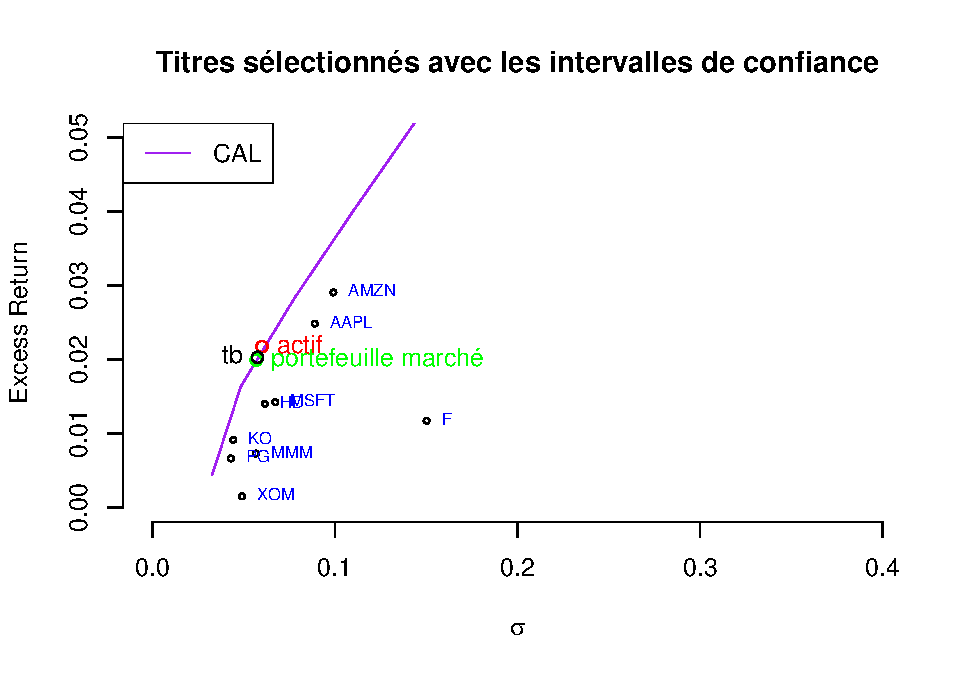
\includegraphics[width=0.5\linewidth]{TP-3_files/figure-latex/unnamed-chunk-22-1}
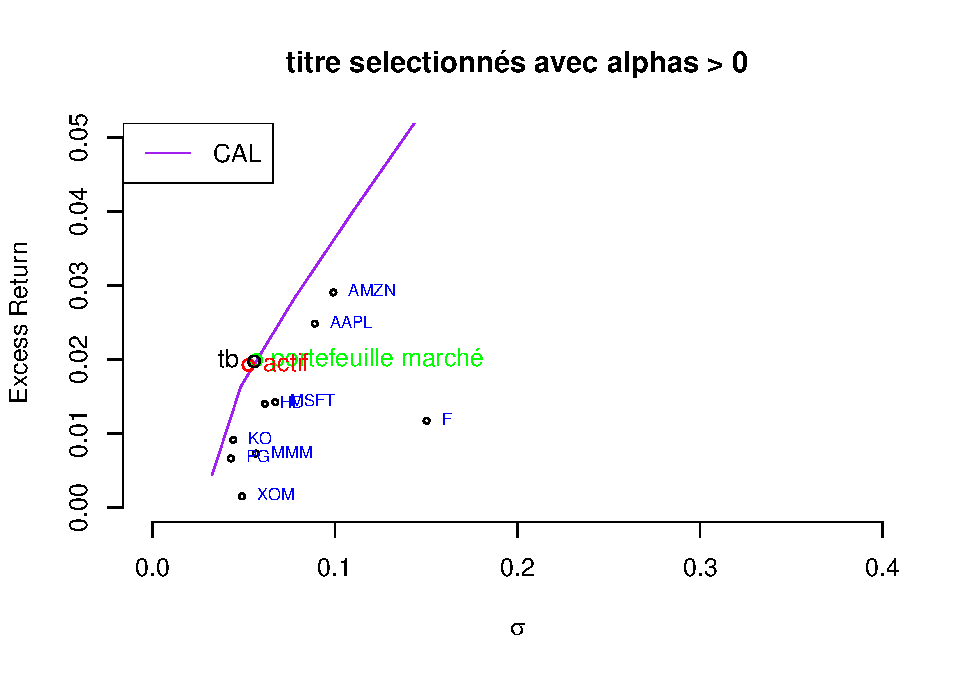
\includegraphics[width=0.5\linewidth]{TP-3_files/figure-latex/unnamed-chunk-22-2}

\end{document}
